\label{sec:algorithm-pixmap-monochrome}

Obraz monochromatyczny to obraz w odcieniach szarości, od białego do czarnego lub od czarnego do białego. Dane są zapisane w sposób ciągły wartość po wartości.

\subsubsection{Pseudokolorowanie obrazu}

Mamy obraz, którego piksele to n-bitowe liczby, na przykład 16 bitowa liczba całkowita.
W takiej postaci wyświetlemoe obrazu na monitorze RGB lub nawet na profesjonalnym 10-bitowym jest niemożliwe.
Należy taką liczbę przerobić na trzy liczby, reprezentujące 3 kanały RGB, czerwony, zielony i niebieski.
Dlatego do wyświetlania obrazów monochromatycznych o dużym kontraście stosuję się twór zwany okienkiem.
Jest to funkcja, która mapuje n-bitwy obraz na 8-bitowy obraz w skali szarości.
8-bitów, ponieważ monitor RGB jest wstanie wyświetlić 256 odcieni szarości.

\paragraph*{Zwiększanie kontrastu za pomocą \enquote{funckji okna}}
Jest przyjęte, że \enquote{okno} definiuje się dwoma liczbami: środkiem, oznaczanym jako $center$ i długością, oznaczaną jako $width$.
Wyznaczamy zakres okienka $x_0$ i $x_1$ ze środka okienka $center$ i długości $width$.
\[x_0 = center - width / 2\]
\[x_1 = center + width / 2\]
Wyznaczamy parametry $a$ i $b$, prostej przechodzącej przez dwa punkty $(x_0, y_0)$ i $(x_1, y,_1)$.
Gdzie $y_0$ jest równe 0, a $y_1$ jest równe 255.
Funkcja \enquote{okna} wygląda następująco:
\[
    f(v)=
    \begin{cases}
        0     & \text{gdy $0 \le v \wedge v \le x_0$ } \\
        a*x+b & \text{gdy $x_0 < v \wedge v < x_1$}    \\
        255   & \text{gdy $x_1 \le v \wedge v \le 1$ }
    \end{cases}
\]

gdzie $v$ to wartość piksela danych obrazu.

Następnie iterujemy przez wszystkie woksele obrazu i używamy na nich funkcji \enquote{okna} i otrzymujemy obraz w skali od $0$ do $255$.
Taki obraz w skali można już wyświetlić.
Natomiast standard DICOM przewiduje, że obraz można jeszcze wyświetlić w wielokolorowej palecie barw.
Przykład takiej palety HotIron w porównaniu do skali szarości można zobaczyć na rysunku .
Taka paleta barw nie koniecznie musi mieć 256 odcieni, dlatego lepiej jest zrobić aby \enquote{okno}, mapowało na liczbę od 0 do 1, a później paleta mapowała na kolor RGB.

\begin{figure}[!htbp]
    \centering
    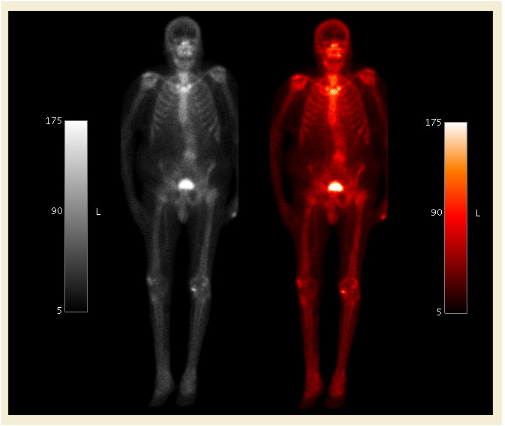
\includegraphics[width=0.7\textwidth]{img/monochrome-001.png}
    \caption{Paleta HotIron (po prawej) w porównaniu do palety w skali szarości (po lewej). Zdjęcie ze standardu DICOM dostępne pod adresem \url{http://dicom.nema.org/medical/dicom/2019a/output/chtml/part06/chapter_B.html}.}
    \label{fig:monochrome1}
\end{figure}

Teraz iterujemy po wszystkich możliwych wartościach wartośćiach obrazu i wykonujemy takie operacje.
\begin{itemize}
    \item wyznaczenie wartości okienka.
          \[y = a * x + b\]
    \item y zostaje obcięcie do 1.0 lub 0.0 jeżeli wyjdzie poza zakres od 1.0 do 0.0
    \item pobranie z palety piksel odpowiadający wartości
    \item wsadzenie piksela do tablicy, tak aby najmniejsza wartości obrazu miała indeks 0 a największy ostani
\end{itemize}


\subsubsection{Implementacja algorytmu}

\paragraph{Opis}
\par
Z uwagi na konieczność osiągnięcia dużej szybkości wyświetlania obrazu, warto jest taksować wartości funkcji f.
Wartości tej funkcji należy przeliczyć, gdy zmienione zostaną parametry tak zwanego \enquote{okna}.
Indeks koloru wyznaczany jest wtedy poprzez pobieranie wartości z tabeli o indeksie równym wartości równym wartości numerycznej w obrazie.
Unikamy w ten sposób wielokrotnego wyznaczania wartości funkcji, która wymaga sprawdzenia warunku, czy dana wartość mieści się w wybranym przedziale wartości, w tan zwanym oknie, co jest bardzo kosztowne obliczeniowo.
Dlatego dobrym pomysłem jest stworzenie mniejszej tablicy typu LookUpTable, wypełnienie jej wszystkimi możliwymi wartościami obrazu, a następnie przerobienie obrazu z tablicą LUT.
Ponieważ tablica LUT posiada wszystkie możliwe kombinacje wartości, jej rozmiar można wyznaczyć wzorem: $2^N*3$, gdzie $N$ to liczba bitów liczby.
Standard \DICOM definiuje, że liczby mogą mieć $8$, $12$, $16$, $32$ i $64$ bity, jednakże, $12$ bitowe i tak się zapisuje w postaci 16-bitowych w pamięci RAM.
Dlatego możliwe wartości wielkości tablicy LUT to w przybliżeniu: $768$ bajtów, $196$ kilobajtów, $12,5$ gigabajtów i $56$ eksabajta ($55*10^{6}$ terabajtów).
Alokowanie dwóch największych wartości może być lekko problematyczne, dlatego w pracy wykonano dwie implementacje algorytmu: z tablicą LUT (dla 8 i 16 bitowych obrazów i bez tablicy LUT (dla 32 i 64 bitowych obrazów).
Algorytm składa się z 3 części: wyznaczenie parametrów \enquote{okna}, przygotowanie \enquote{okna} (tylko gdy jest tablica LUT), wielowątkowa iteracja po obrazie.
\par
Okno z LUT jest implementowane przez \sokarclass{Monochrome{\scopedots}WindowIntStatic}.
Okno bez LUT jest implementowane przez \sokarclass{Monochrome{\scopedots}WindowIntDynamic}.
Obie klasy dziedziczą po abstrakcyjnej klasie \sokarclass{Monochrome}{Window}, która z kolei dziedziczy po \sokarclass{SceneIndicator}, dlatego od razu może wyświetlać obecne wartości \enquote{okna}.
Decyzja o używanym \enquote{oknie} jest podejmowana podczas wczytywania obrazu przez klasę \sokarclass{Monochrome{\scopedots}Scene}
\par
UWAGA: Standard \DICOM zakłada, że danymi mogą być liczby całkowite(\cppcode{int}) oraz zmiennoprzecinkowe(\cppcode{float} lub \cppcode{double}), ale praktycznie, nie ma takich aparatów medycznych, które zapisywały by takie obrazy, gdzie dane to liczby zmiennoprzecinkowe.
Dlatego w pracy założono, że takie obrazy nie będą obsługiwane.

\paragraph{Wyznaczenie parametrów okna}
\par
Najpierw wyznaczam okienko, które zmienia wartości obrazu na skale od zera do jeden:
\[x_0 = center - width / 2\]
\[x_1 = center + width / 2\]
\[y_1 = 0.0\]
\[y_0 = 1.0\]
gdzie:
\begin{itemize}
    \item $center$ --- środek okienka
    \item $width$ --- szerokość okienka
    \item $x0$ i $y0$ --- współrzędne pierwszego punktu
    \item $x1$ i $y1$ --- współrzędne drugego punktu
\end{itemize}
Przeglądarka pozwala na inwersje okienka.
Dlatego kiedy użytkownik zażyczy sobie inwersji, zmienne $y0$ i $y1$ zamienią się wartoścami.

Standard \DICOM przewiduje, że wszystkie dane powinny być wyskalowane, za pomocą wzoru.
\[OutputUnits = m*SV + b\]
gdzie:
\begin{itemize}
    \item $m$ --- wartość z \dicomtag{RescaleSlope}{0028}{1053}
    \item $b$ --- wartość z \dicomtag{RescaleIntercept}{0028}{1052}
    \item $SV$ --- stored values --- warość pixela z pliku
    \item $OutputUnits$ --- wartość wynikowa
\end{itemize}

Wartości okienka odnoszą się do wartości już wyskalowanej, a ponieważ skalowanie całego obrazu jest czasochłonne, przeskalowaie okienka da taki sam efekt:
\[(OutputUnits - b ) / m = SV \]
więc:
\[x_0 -= rescaleIntercept\]
\[x_1 -= rescaleIntercept\]
\[x_0 /= rescaleSlope\]
\[x_1 /= rescaleSlope\]

Posiadamy, teraz dwa punkty okienka odnoszące się do wartośći obrazu.
Wyznaczono parametry prostej przechodzącej przez dwa punkty:
\[a = (y_1 - y_0) / (x_1 - x_0)\]
\[b = y_1 - a * x_1\]

\par
Teraz algorytm się rozdwaja.
Pobieranie wartości z okienka odbywa się za pomocą funkcji \sokarclass{Monochrome}{Window\zerospace::{\zerospace}getPixel()}.

\paragraph{Implementacja dynamiczna bez tablicy LUT}

\par
W tej wersji funkcja \sokarfunction{Monochrome{\scopedots}Window}{getPixel} wygląda następująco:
\par
\begin{lstlisting}
inline const Pixel &getPixel(quint64 value) override {
    if (value < x0) {
        return background;
    } else if (value > x1) {
        return foreground;
    } else {
        return palette->getPixel(a * value + b);
    }
}
\end{lstlisting}
\par
Widzimy tutaj, że funkcja najpierw sprawdza czy zakres okienka został przekroczony, następnie wylicza wartość obrazu i pobiera kolor z palety.
\par
UWAGA: ponieważ nie istnieją rzeczywiste obrazy o wokselu 32-bitowym lub 64-bitowym, implementacja dynamiczna nie była testowana w warunkach rzeczywistych.

\paragraph{Implementacja statyczna z tablicą LUT}
\par
W wersji z LUT, podczas tworzenia okienka jest alokowany wektor obiektów \sokarclass{Pixel} klasy \stdclass{vector}{container/vector}.
Standard \DICOM przewiduje, że woksele mogą mieć wartości ujemne, więc tablica powinna mieć możliwość posiadania takich wartości indeksów, ale C++ nie przewiduje takiej możliwości.
Dlatego wprowadzono dwie zmienne pomocnicze \cppcode{maxValue} i \cppcode{signedMove}.
\cppcode{maxValue} jest to maksymalna wartość jaką dane mogą przyjąć, jest ona równa $2^N$, gdzie $N$ to liczba bitów brana z \dicomtag{BitsStored}{0028}{0101}.
A \cppcode{signedMove} to liczba przesunięcia liczb, przyjmuje wartość zero, gdy dane wokseli są całkowite nieujemne lub wartość przeciwną do \cppcode{maxValue}, gdy woksele są być ujemne.
Długość wektora pikseli jest sumą \cppcode{maxValue} i \cppcode{signedMove}.
A indeks woksela w wektorze ma wartość tego woksela zwiększoną o \cppcode{signedMove}.
\par
Wypełnienie wektora wartościami odbywa się poprzez iteracje po wszystkich możliwych wartościach, przeliczenie ich przez funkcje \enquote{okna}, a następnie wstawienie ich do wektora.
W celu poprawy szybkości, zastosowano sprawdzanie czy wartości są w zakresie \enquote{okna}.
Poniżej kod funkcji:
\begin{lstlisting}
bool genLUT() override {

    if (WindowInt::genLUT()) {

        /* Przeskalowanie wektora, gdy jest to wymagane */
        if (arraySize != signedMove + maxValue) {
            arraySize = signedMove + maxValue;
            arrayVector.resize(arraySize);
        }

        /* Wyliczenie najmniejszej wartości */
        qreal x = qreal(signedMove) * -1;

        auto &background = isInversed() ? palette->getForeground() : palette->getBackground();
        auto &foreground = isInversed() ? palette->getBackground() : palette->getForeground();

        /* Iteracja */
        pixelArray = &arrayVector[0];
        for (int i = 0; i <= arraySize; i++) {

            if (x < x0) {
                *pixelArray = background;
            } else if (x > x1) {
                *pixelArray = foreground;
            } else {
                *pixelArray = palette->getPixel(a * x + b);
            }

            x++;
            pixelArray++;
        }

        pixelArray = &arrayVector[0];

        updateLastChange();

        return true;
    }
    return false;
}
\end{lstlisting}

\par
Funkcja zmiany wartości obrazu na kolor prezentuje się następująco:
\begin{lstlisting}
inline const Pixel &getPixel(quint64 value) override {
    return *(pixelArray + signedMove + value);
}
\end{lstlisting}

\paragraph{Iterowanie po obrazie}
\par
Po wygenerowania obraz, należy przeiterować go przez funkcje \enquote{okna}.
Do zokienkowania jednego piksela nie potrzeba innego piksela dlatego w celu przyspieszenia procesu okienkowania, iteracja po obrazie odbywa się w wielu wątkach.
\par
W C++ typy zmiennych muszą być zdefiniowane przed kompilacją, co jest bardzo problematyczne.
Mając dwa typy okienek, każde odsługujące 4 typy liczb całkowitych, musiało by zostać zaimplementowanych 8 prawie identycznych funkcji.
Dlatego podział ten został zaimplementowany za pomocą 4 funkcji z szablonami:
\begin{itemize}
    \item \sokarfunction{Monochrome{\scopedots}Scene}{genQPixmapOfTypeWidthWindowThread}

          Jest funkcją jednego wątku, który iteruje po obrazie.
          Jego parametrami są zakresy podane w indeksach wokseli po któych ma iterować.
          \cppcode{IntType} to jest typ zmiennej woksela obrazu.
          \cppcode{WinClass} klasa okienka.
          Nazewnictwo będzie kontynuowane w następnych punktach.
          Kod funkcji:
          \begin{lstlisting}
template<typename IntType, typename WinClass>
void Monochrome::Scene::genQPixmapOfTypeWidthWindowThread(quint64 from, quint64 to) {

    auto buffer = &targetBuffer[from];
    auto origin = (IntType *) &originBuffer[0];
    auto windowPtr = (WinClass *) getCurrentWindow();

    origin += from;

    for (quint64 i = from; i < to; i++, origin++) {
        /* W tym miejscu jest dokonywana zamiana liczby na kolor */
        *buffer++ = windowPtr->getPixel(*origin);
    }
}
\end{lstlisting}

    \item \sokarfunction{Monochrome{\scopedots}Scene}{genQPixmapOfTypeWidthWindow}

          Jest to funkcja, która dzieli obraz na wątki, tworzy je i uruchamia.
          Ilość wątków jest ustalana za pomocą funkcji \qtfunction{QThread}{idealThreadCount}.
          Wątki działają na zakresach o długości ilości wokseli podzielonej przez ilość wątków.
          Kod funkcji:
          \begin{lstlisting}
template<typename IntType, typename WinClass>
void Monochrome::Scene::genQPixmapOfTypeWidthWindow() {

    /* Tworzenie wektora wątków */
    std::vector<std::thread> threads;

    quint64 max = imgDimX * imgDimY;
    quint64 step = max / QThread::idealThreadCount();

    for (int i = 1; i < QThread::idealThreadCount(); i++) {
        std::thread t(&Scene::genQPixmapOfTypeWidthWindowThread<IntType, WinClass>,
                      this,
                      i * step,
                      std::min((i + 1) * step, max));

        threads.push_back(std::move(t));
    }

    /* W celu zmniejszenia ilości wątków, wątek obecny też zostanie wykorzystany */
    genQPixmapOfTypeWidthWindowThread<IntType, WinClass>(0, step);

    /* Czekanie na wszystkie wątki */
    for (auto &t: threads) t.join();
}
\end{lstlisting}

    \item \sokarfunction{Monochrome{\scopedots}Scene}{genQPixmapOfType}

          Jest to funkcja pomocnicza ustalająca obecną klasę obecnego \enquote{okna}, aby móc wykonać funkcje \sokarfunction{Monochrome{\scopedots}Scene}{genQPixmapOfTypeWidthWindow}.
          Kod funkcji:
          \begin{lstlisting}
template<typename IntType>
void Monochrome::Scene::genQPixmapOfType() {

    switch (getCurrentWindow()->type()) {
        case Window::IntDynamic:
            genQPixmapOfTypeWidthWindow<IntType, WindowIntDynamic>();
            break;

        case Window::IntStatic:
            genQPixmapOfTypeWidthWindow<IntType, WindowIntStatic>();
            break;

        default:
            throw WrongScopeException(__FILE__, __LINE__);
    }
}
\end{lstlisting}

    \item \sokarfunction{Monochrome{\scopedots}Scene}{generatePixmap}

          Funkcja odświeża okienko i sprawdza, czy odświeżenie obrazu jest konieczne, następnie sprawdza typ liczby woksela i uruchamia \sokarfunction{Monochrome{\scopedots}Scene}{genQPixmapOfType}.
          Kod funkcji:
          \begin{lstlisting}
bool Monochrome::Scene::generatePixmap() {

    /* Odświeżamy okno i sprawdzamy czy odświeżenie obrazu jest konieczne */
    getCurrentWindow()->genLUT();
    if (lastPixmapChange >= getCurrentWindow()->getLastChange()) return false;

    /* Sprawdzamy typ liczby woksela obrazu */
    switch (gdcmImage.GetPixelFormat()) {
        case gdcm::PixelFormat::INT8:
            genQPixmapOfType<qint8>();
            break;
        case gdcm::PixelFormat::UINT8:
            genQPixmapOfType<quint8>();
            break;
        case gdcm::PixelFormat::INT16:
            genQPixmapOfType<qint16>();
            break;
        case gdcm::PixelFormat::UINT16:
            genQPixmapOfType<quint16>();
            break;
        case gdcm::PixelFormat::INT32:
            genQPixmapOfType<qint32>();
            break;
        case gdcm::PixelFormat::UINT32:
            genQPixmapOfType<quint32>();
            break;
        case gdcm::PixelFormat::INT64:
            genQPixmapOfType<qint64>();
            break;
        case gdcm::PixelFormat::UINT64:
            genQPixmapOfType<quint64>();
            break;

        default: /* W przypadku innych jest zwracany wyjątek */
            throw Sokar::ImageTypeNotSupportedException();
    }

    pixmap.convertFromImage(qImage);
    return true;
}
\end{lstlisting}
\end{itemize}

\subsubsection{Palety}
Klasa \sokarclass{Palette} reprezentuje palety kolorów używanych do pseudokolorwania obrazu.
Paleta przerabia liczbę zmiennoprzecinkową od zera do jedynki na kolor RGB, zwracając \sokarclass{Pixel}.
Paleta nie ma zdefiniowanej długości minimalnej i maksymalnej.

\par
Palety są wczytywane z plików XML w czasie uruchamiania programu i można definiować własne palety nie będące częścią standardu.
Przykładowy wygląd pliku palety HotIron:
\begin{lstlisting}[language=XML]
<palette display="Hot Iron" name="HOT_IRON">

    <entry red="0" green="0" blue="0"/>
    <entry red="2" green="0" blue="0"/>
    <entry red="4" green="0" blue="0"/>

    ...

    <entry red="254" green="0" blue="0"/>
    <entry red="255" green="0" blue="0"/>
    <entry red="255" green="2" blue="0"/>

    ...

    <entry red="255" green="250" blue="248"/>
    <entry red="255" green="252" blue="252"/>
    <entry red="255" green="255" blue="255"/>
</palette>
\end{lstlisting}